\subsection{Vectors and physics}

Suppose you push
on something. Then, your push is made up of two components, how hard you push and the direction you push. This illustrates the concept of force.

\begin{definition}{Force}{force}
\textbf{Force}\index{force} is a vector. The magnitude of this vector is a measure of how
hard it is pushing. It is measured in Newtons\index{Newton}. The direction of this vector is the direction in which the push is taking place.
\end{definition}

Vectors are used to model force and other physical vectors like velocity.
 As with all vectors, a vector modelling force has two essential
ingredients, its magnitude and its direction.

Recall the special vectors which point along the coordinate axes.
These are given by 
\begin{equation*}
\vect{e}_{i} = \mat{0,\ldots,0,1,0,\ldots,0}^T
\end{equation*}
where the $1$ is in the $i^{th}$ slot and there are zeros in all the other
spaces. The direction of $\vect{e}_{i}$ is referred to as the $i^{th}$ direction.

Consider the following picture which illustrates the case of $\R^{3}$. 
Recall that in $\R^3$, we may refer to these vectors as $\vect{i}, \vect{j}$, and $\vect{k}$. 

\begin{center}
\begin{tikzpicture}
\draw(0,0,2.5)--(0,0,0)--(0,0,-2);
\draw(-2,0,0)--(0,0,0)--(2,0,0);
\draw(0,-2,0)--(0,0,0)--(0,2,0);
\draw[ultra thick, ->, red](0,0,0)--(0,0,1.5);
\draw[ultra thick, ->, blue](0,0,0)--(0,1,0);
\draw[ultra thick, ->, green](0,0,0)--(1,0,0);
\node[left] at (0,0,2.5){$x$};
\node[below] at (2,0,0){$y$};
\node[above] at (0,2,0){$z$};
\node[left] at (-0.2,0,1){$\vect{e}_1$};
\node[below] at (1,0,0){$\vect{e}_2$};
\node[left] at (0,1,0){$\vect{e}_3$};
\end{tikzpicture}
\end{center}

Given a vector $\vect{u}=\mat{u_{1},\ldots,u_{n}}^T$, it follows
that
\begin{equation*}
\vect{u}=u_{1}\vect{e}_{1}+\ldots +u_{n}\vect{e}_{n}=
\sum_{k=1}^{n}u_{i}\vect{e}_{i}
\end{equation*}

What does addition of vectors mean physically? Suppose two forces are
applied to some object. Each of these would be represented by a force vector
and the two forces acting together would yield an overall force acting on
the object which would also be a force vector known as the
resultant\index{resultant}. Suppose the two vectors are $\vect{u}=\sum_{k=1}^{n}u_{i}\vect{e}_{i}$ and $\vect{v}=\sum_{k=1}^{n}v_{i}\vect{e}_{i}$. Then the vector $\vect{u}$ involves a component in the $
i^{th}$ direction given by $u_{i}\vect{e}_{i}$, while the component in the $i^{th}$
direction of $\vect{v}$ is $v_{i}\vect{e}_{i}$. Then the vector $\vect{u} + \vect{v}$ should have a component in the $i^{th}$
direction equal to $(u_{i}+v_{i}) \vect{e}_{i}$. This is
exactly what is obtained when the vectors, $\vect{u}$ and $\vect{v}$ are
added.
\begin{eqnarray*}
\vect{u}+\vect{v}& =&\mat{u_{1}+v_{1},\ldots,u_{n}+v_{n}}^T  \\
& =&\sum_{i=1}^{n}(u_{i}+v_{i}) \vect{e}_{i}
\end{eqnarray*}

Thus the addition of vectors according to the rules of addition in $\R^{n}$ which were presented earlier, yields the appropriate vector which
duplicates the cumulative effect of all the vectors in the sum.

Consider now some examples of vector addition.

\begin{example}{The resultant of three forces}{resultant-three-forces}
There are three ropes attached to a car and three people pull on these
ropes. The first exerts a force of $\vect{F}_1 = 
2\vect{i} + 3\vect{j} -2 \vect{k}$ Newtons, the second exerts a force of $\vect{F}_2
=
3\vect{i}+5\vect{j}+\vect{k}$ Newtons
and the third exerts a force of $5\vect{i}-\vect{j}+2\vect{k}$ Newtons. Find
the total force in the direction of $\vect{i}$.
\end{example}

\begin{solution}
To find the total force, we add the vectors as described above. 
This is given by 
\begin{eqnarray*}
&&(2\vect{i}+3\vect{j}-2\vect{k}) + (3\vect{i}+5\vect{j}+\vect{k}) + (5\vect{i}-\vect{j}+2\vect{k})\\
&=&
(2  + 3 + 5) \vect{i} + (3 + 5 + -1) \vect{j} + (-2+1+2) \vect{k} \\
&=&
10 \vect{i} + 7 \vect{j} + \vect{k}
\end{eqnarray*}
Hence, the total force is  $10\vect{i}+7\vect{j}+\vect{k}$ Newtons. Therefore, the force in the $
\vect{i}$ direction is $10$ Newtons.
\end{solution}

Consider another example.

\begin{example}{Finding a vector from geometric description}{vector-from-geometric-description}
An airplane flies North East at $100\textrm{km}/\textrm{h}$. Write this as a vector.
\end{example}

\begin{solution}
A picture of this situation follows.

\begin{center}
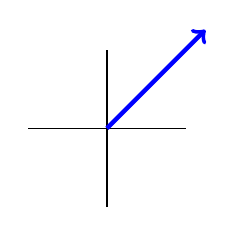
\begin{tikzpicture}[scale=0.5]
\draw(-2,0)--(2,0);
\draw(0,-2)--(0,2);
\draw[ultra thick, ->, blue](0,0)--(2.5,2.5);
\end{tikzpicture}
\end{center}

Therefore, we need to find the vector $\vect{u}$ which has length 100 and direction as shown in this diagram. 
We can consider the vector $\vect{u}$ as the hypotenuse of a
right triangle having equal sides, since the direction of $\vect{u}$ corresponds with the $45 ^{\circ}$ line. 
The sides, corresponding to the $\vect{i}$ and $\vect{j}$ directions,  should be each of length 100/$
\sqrt{2}$. Therefore, the vector is given by 
\[
 \vect{u} = \frac{100}{\sqrt{2}} \vect{i}+ \frac{100}{\sqrt{2
}}\vect{j}
=
\begin{mymatrix}{rr}
\vspace{0.05in} \frac{100}{\sqrt{2}} & \vspace{0.05in}\frac{100}{\sqrt{2}}
\end{mymatrix}^T\
\]
\end{solution}

This example also motivates the concept of \textbf{velocity}, defined below.

\begin{definition}{Speed and velocity}{speed-velocity}
The \textbf{speed}\index{speed} of an object is a measure of how fast it is going. It is
measured in units of length per unit time. For example, kilometers per
hour, meters per second. The
\textbf{velocity}\index{velocity} is a vector having the speed as the
magnitude but also specifying the direction.
\end{definition}

Thus the velocity vector in the above example is $\vspace{0.05in}\frac{100}{\sqrt{2}}\vect{i}+
\vspace{0.05in}\frac{100}{\sqrt{2}}\vect{j}$, while the speed is $100\textrm{km}/\textrm{h}$.

Consider the following example. 

\begin{example}{Position from velocity and time}{position-velocity-time}
The velocity of an airplane is $100\vect{i}+\vect{j}+\vect{k}$
measured in kilometers per hour and at a certain instant of time its
position is $(1,2,1)$. 

Find the position of this airplane one minute later.
\end{example}

\begin{solution}
Here imagine a Cartesian coordinate
system in which the third component is altitude and the first and second
components are measured on a line from West to East and a line from South to
North. 

Consider the vector $
\begin{mymatrix}{rrr}
1 & 2 & 1
\end{mymatrix}^T$, which is the initial position vector
of the airplane. As the plane moves, the position vector changes according to the velocity vector. 
After one minute (considered as $\frac{1}{60}$ of an hour)
the airplane has moved in the $\vect{i}$ direction a distance of 
$100\times \frac{1}{60}= \frac{5}{3}$ kilometer. In the $\vect{j}
$ direction it has moved $\frac{1}{60}$ kilometer during this same time,
while it moves $\frac{1}{60}$ kilometer in the $\vect{k}$ direction.
%\begin{picture}(1,425)\end{picture}
Therefore, the new displacement vector for the airplane is
\begin{equation*}
\begin{mymatrix}{rrr}
1 & 2 & 1
\end{mymatrix}^T +
\begin{mymatrix}{rrr}
\frac{5}{3} & \frac{1}{60} & \frac{1}{60}
\end{mymatrix}^T
=\begin{mymatrix}{rrr}
\frac{8}{3} & \frac{121}{60} & \frac{121}{60}
\end{mymatrix}^T
\end{equation*}
\end{solution}

Now consider an example which involves combining two velocities.

\begin{example}{Sum of two velocities}{sum-of-two-velocities}
A certain river is one half kilometer wide with a current flowing at 4 kilometers per
hour from East to West. A man swims directly toward the opposite shore from
the South bank of the river at a speed of 3 kilometers per hour. How far down the
river does he find himself when he has swam across? How far does he end up
swimming?
\end{example}

\begin{solution}
Consider the following picture which demonstrates the above scenario. 

\begin{center}
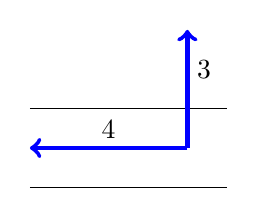
\begin{tikzpicture}[scale=0.5]
\draw(-3,1)--(2,1);
\draw(-3,-1)--(2,-1);
\draw[ultra thick, blue, ->](1,0)--(-3,0);
\draw[ultra thick, blue, ->](1,0)--(1,3);
\node[above] at (-1,0){$4$};
\node[right] at (1,2){$3$};
\end{tikzpicture}
\end{center}

First we want to know the total time of the swim across the river. 
The velocity in the direction across the river is
$3$ kilometers per hour, and the river is $\frac{1}{2}$ kilometer wide. It follows the trip
takes $1/6$ hour or $10$ minutes. 

Now, we can compute how far downstream he will end up. Since the river runs at a rate of 
$4$ kilometers per hour, and the trip takes $1/6$ hour, the distance travelled downstream 
is given by $4 \paren{\frac{1}{6}} = \frac{2}{3}$ kilometers. 

The distance travelled by the swimmer is given by the hypotenuse of a right triangle. 
The two arms of the triangle are given by the distance across the river, $\frac{1}{2}$km, and 
the distance travelled downstream, $\frac{2}{3}$ km. Then, using the Pythagorean Theorem, we can calculate
the total distance $d$ travelled.
\begin{equation*}
d
=
\sqrt{ \paren{\frac{2}{3}}^2 + \paren{\frac{1}{2}} ^2 }
=
\frac{5}{6} \mbox{km}
\end{equation*}

Therefore, the swimmer travels a total distance of $\frac{5}{6}$ kilometers. 
\end{solution}
